\chapter{Introduction}

\section{Background}
The energy sector is undergoing significant change, with a decline in fossil fuel use and a rise in renewable energy sources such as solar, nuclear, hydro, and wind energy (\cite{IEA2024}). By 2023, renewable energy represented almost 15\% of total energy production (\cite{EnergyInstitute2024}). To achieve zero emissions by 2025, these renewable resource areas need to be increased significantly.

Wind energy utilises the kinetic energy of wind to generate electricity. As a clean and sustainable option, it is one of the fastest-growing segments of the global energy market. Recent advancements in wind turbine design and materials have enhanced energy capture efficiency and reduced the levelized cost of electricity (LCOE) for wind energy production (\cite{GWEC2024}; \cite{GWEC2024Offshore}). These improvements result from scaling up production, increasing turbine sizes, and lowering installation and maintenance costs.

Establishing both onshore and offshore wind farms is needed to diversify the energy mix and to meet climate goals (\cite{IEA2024}). Offshore wind energy is especially significant because these farms benefit from faster and more consistent wind patterns compared to onshore installations (\cite{GWEC2024Offshore}). This leads to higher capacity factors,  greater energy production potential, and reduced operational costs (\cite{GWEC2024}). In addition, offshore wind turbines generally face fewer space and noise restrictions, allowing larger installations with less impact on local communities.

The global offshore wind industry is entering a new phase of growth, marked by record installations and supportive policies that drive future development (\cite{GWEC2024}). In 2023, the offshore wind sector had an operational capacity of 75 GW, in 2028 this is forecasted to be tripled (\cite{GWEC2024Offshore}). This sector also generates jobs and boosts economic growth in coastal regions (\cite{GWEC2024}).

To realize the full potential of offshore wind energy, accurate weather forecasting is essential for effective planning and installation of wind turbines. Met-ocean conditions, such as significant wave height, mean wave frequency, and wind speed, greatly influence the feasibility and efficiency of offshore projects. The vessels used in the installation phase operate within specific weather windows, which consist of multiple parts: loading components onto the vessel, transporting them to the site, and assembling them at sea, as can be seen in Figure \ref{fig:installation_process}.

\begin{figure}[h!]
\centering
\begin{tikzpicture}[>=stealth, node distance=5cm, on grid]

\tikzstyle{phase} = [rectangle, rounded corners, draw=black, fill=blue!10, 
                     text centered, text width=3.5cm, minimum height=2cm]

\node[phase] (loading) {
  \textbf{Loading} \\
  \footnotesize Components loaded \\
  \footnotesize onto vessel \\
};

\node[phase, right=of loading] (transit) {
  \textbf{Transit} \\
  \footnotesize Vessel at sea \\
};

\node[phase, right=of transit] (assembly) {
  \textbf{Assembly} \\
  \footnotesize Turbine \\
  \footnotesize installation \\
};

\draw[->, thick] (loading) -- (transit);
\draw[->, thick] (transit) -- (assembly);

\end{tikzpicture}
\caption{Overview of the offshore wind turbine installation process}
\label{fig:installation_process}
\end{figure}

\newpage
These tasks are carried out by different vessels that will be limited by the met-ocean conditions. Using advanced forecasting methods, developers can better predict and manage installation timelines, ultimately reducing delays caused by adverse weather. Moreover, accurate forecasting can optimise wind turbine placement and design, ensuring that installations are tailored to local conditions for maximum output. This precision helps to achieve better project results and ensures safer offshore operations. From an economic standpoint, when delays occur, vessels must still be rented while no installation occurs, leading to increased costs.

Understanding and predicting met-ocean conditions will help to capture risks associated with installation and operation. So, enhancing the overall performance of wind energy systems. By integrating reliable forecasting into the planning stages, the offshore wind sector can make informed decisions. This will lead to less delays and so an overall more efficient installation process (\cite{IEA2021}; \cite{GWEC2024Offshore}).

\section{Problem Statement}
Offshore wind farms are an essential part of the transition towards renewable energy. However, ocean conditions often ground specialized installation vessels, along with their crews, as they wait for safe weather to load, transport and assemble wind turbine components at sea. These delays can quickly increase project costs and potentially damage equipment if wave conditions or wind speeds go above forecast thresholds (\cite{Boccaletti2019}; \cite{Kelley2018}).

Although the stakes are high, current forecasting methods fall short in two main areas. First, many techniques lack sufficient accuracy for dynamic offshore environments, where complex wave, wind, and atmospheric interactions are interdependent (\cite{Murphy1993}; \cite{Wilks2011}). Second, most models often cannot quickly adapt to local changes, leaving operators with inaccurate predictions during the installation windows. This makes it easy to underestimate a storm or miscalculate the frequency of wave activity, with the safety of crew and project schedules at risk.

In response, researchers started experimenting with more advanced models, ranging from hybrid and probabilistic approaches to deep learning techniques (\cite{Zhang2019}; \cite{Huang2020}). However, there remains a need to compare these methods side by side under realistic offshore scenarios and changing refit intervals. This comparison aims to determine which model best balances accuracy, reliability, and practicality.

 The research investigates three advanced forecasting strategies: a Bayesian Neural Network with Monte Carlo Dropout, an LSTM-based deep learning approach, and a Hybrid ARIMA–ANN model. Focusing on significant wave height, mean wave frequency, and wind speed. By evaluating how each parameter performs under real data conditions, this research aims to reduce weather-related project delays and streamline the installation of offshore wind turbines. The process is visualized in Figure \ref{fig:forecast_process}. The objective is to lower operational costs but also enhance safety for those working in the renewable energy sector. 

\begin{figure}[h!]
    \centering
    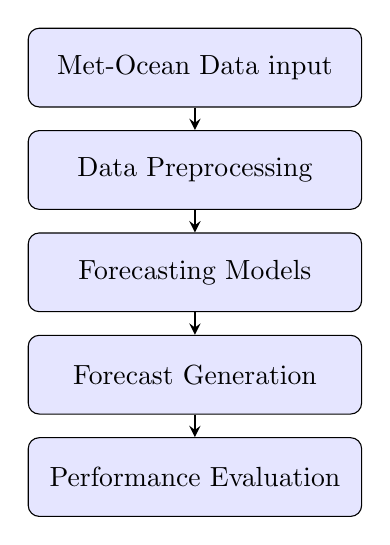
\begin{tikzpicture}[node distance=1.3 cm, auto]

    \tikzstyle{block} = [rectangle, draw, fill=blue!10, rounded corners, text width=4 cm, text centered, minimum height=1 cm]
    \tikzstyle{arrow} = [thick,->,>=stealth]
    
    \node[block] (data) {Met-Ocean Data input};
    \node[block, below of=data] (preprocessing) {Data Preprocessing};
    \node[block, below of=preprocessing] (models) {Forecasting Models};
    \node[block, below of=models] (forecast) {Forecast Generation};
    \node[block, below of=forecast] (evaluation) {Performance Evaluation};
    
    \draw[arrow] (data) -- (preprocessing);
    \draw[arrow] (preprocessing) -- (models);
    \draw[arrow] (models) -- (forecast);
    \draw[arrow] (forecast) -- (evaluation);
    
    \end{tikzpicture}
    \caption{Flow diagram of the forecasting process used in this research.}
    \label{fig:forecast_process}
\end{figure}

 
\section{Research Question and Sub-questions}
To effectively address the challenges associated with weather forecasting for offshore wind turbine installation, research questions are formulated. This study will investigate how various forecasting models can enhance the accuracy of weather predictions, thereby ensuring a more streamlined installation process. 

\subsection*{Research Question}  
How can weather forecasts for significant wave height, mean wave frequency, and wind speed be improved for offshore wind turbine installations by comparing hybrid, probabilistic, and deep learning models, and what is the impact of varying refit intervals on forecast performance?

\subsection*{Sub-questions}
\begin{enumerate}
    \item What are the strengths and limitations of hybrid, probabilistic, and deep learning models for forecasting key weather conditions in offshore wind turbine installation?
    \item How do the BNN with Monte Carlo Dropout, LSTM, and Hybrid ARIMA–ANN compare in forecasting significant wave height, wave frequency, and wind speed using a 5-day refit interval?
    \item How does the Hybrid ARIMA–ANN model’s performance change with varying refit intervals, when the model is retrained with the actual past data (6 hours, 12 hours, 1 day, 2 days, 3 days, 4 days, 5 days, 6 days, 7 days, 1 week, 2 weeks and 4 weeks)?
    \item What are the implications of these forecasting models and intervals for scheduling and risk management in offshore wind farm installation?
\end{enumerate}

\section{Objectives and Scope}
This report aims to improve the accuracy of weather forecasts for offshore wind turbine installations by exploring and comparing various forecasting models. The research's aim and boundary limits will be shown.

\subsection*{Objective}
The primary objective is to enhance the accuracy of weather forecasts to improve the planning and installation of offshore wind turbines. To ensure this objective is met, the research focuses on the following specific aims:

\begin{itemize}
    \item Evaluating and comparing the performance of a Bayesian Neural Network with Monte Carlo Dropout, an LSTM-based deep learning model, and a Hybrid ARIMA–ANN model under a fixed 5-day refit interval. 
    \item Investigating how varying refit intervals (6 hours, 12 hours, 1 day, 2 days, 3 days, 4 days, 5 days, 6 days, 7 days, 1 week, 2 weeks and 4 weeks) affect the performance of the Hybrid ARIMA–ANN model. 
    \item Assessing forecasting accuracy using metrics such as $MSE$, $MAE$, $RMSE$ and $R^2$, alongside visual validation through time series plots, residual distributions and error comparisons.
    \item Analysing the implications of improved forecasting on installation scheduling, risk management, and operational costs.
\end{itemize}

\newpage 

\subsection*{Scope}
The scope of this report is primarily focused on the development and evaluation of forecasting models applicable to offshore wind energy projects, utilizing met-ocean data from a single location over 10 years. While this specific location will be analysed using different models, the findings can be used as a foundation for further multi-site research. Certain parts fall out of the scope of the research:

\begin{itemize}
    \item The focus will be on only three parameters: significant wave height ($s_{wht}$), mean wave frequency ($mean_{fr}$) and wind speed ($wind_{speed}$). These parameters are evaluated; however, additional factors such as wind direction, tides, and swells may also influence the installation phase. 
    \item Only the three forecasting models, BNN with MC dropout, LSTM and Hybrid ARIMA-ANN, are compared. There are other models available.
    \item The evaluation is only based on the data of the installation site and so there is no evaluation possible based on this data for the transportation from the harbour to the site.
    \item Due to computational constraints, model architectures were adjusted by limiting hyper-parameter tuning and reducing training complexity, which may impact their performance compared to fully optimized versions.
    \item This research evaluates forecasting performance based on historical met-ocean data but does not implement real-time model deployment or assess operational feasibility in an active offshore wind installation
\end{itemize}

It is anticipated that the comparative analysis will identify the most robust forecasting approach, thereby providing insights that can reduce weather-related delays and so lower operational costs, and improve the process of offshore wind turbine installations.
